\chapter{UPC Cablecom's Business}
In this chapter we will present the specificities of the company both in terms of network architecture, identified problems, data sources, and setup of the project.

\section{Hybrid Fiber-Coaxial Architecture}
\label{sec:HFC_archi}
Introduced in the 1990s, the Hybrid fiber-coaxial (HFC)\cite{wiki:hfc} architecture describes a broadband network that combines optical fiber and coaxial cable. While it isn't necessary to understand the entire network for this project, we will introduce  a high-level picture of the network as some notions will be required later on to explain some terms and justify choices. 

\vspace{2 \baselineskip}
The project uses measurements that are polled at different levels of the network to determine the "health" of a CPE. Therefore having a clear picture of the topology of the network will later prove to be useful. 

\begin{figure}[ht]
    \begin{center}
    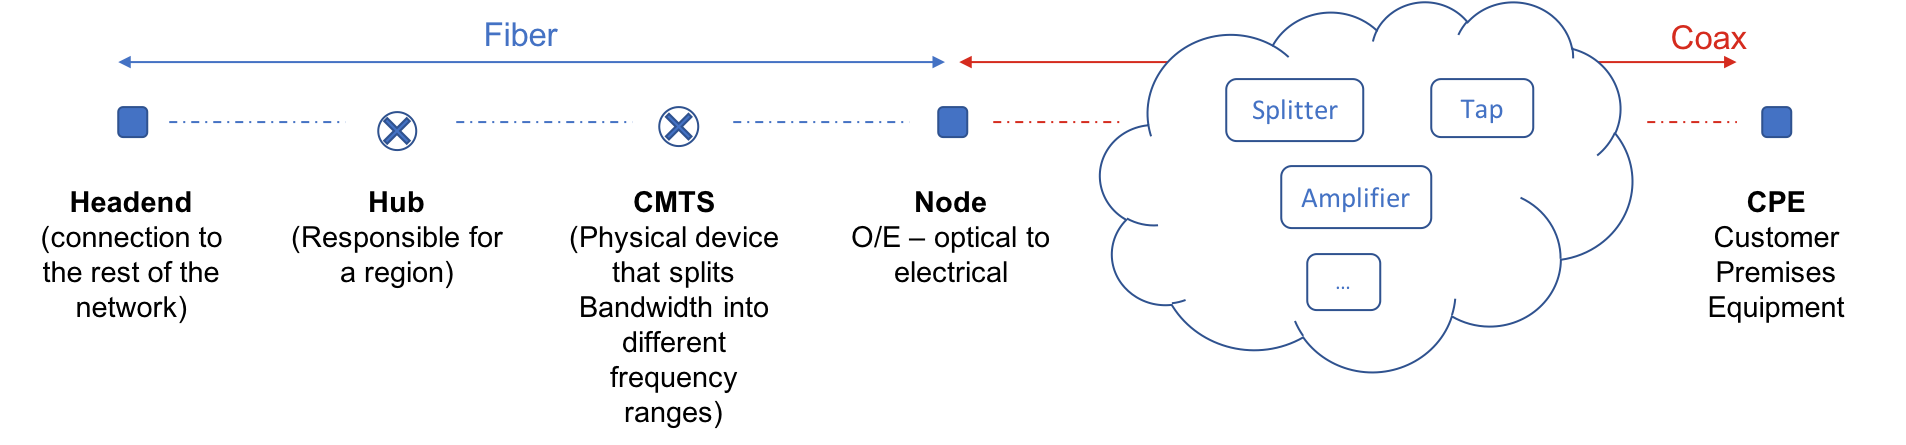
\includegraphics[width=1\linewidth]{HFC}
    \end{center}
    \caption{Hybrid Fiber-Coaxial Topology of the Network}
    \label{HFC}
\end{figure}

Figure~\ref{HFC} illustrates this topology and more specifically how a CPE is connected to the rest of the network. Among nodes that compose the network only two are considered as active and are regularly polled to monitor their behaviour: CPE and CMTS\footnote{Cable Modem Termination System}.

\begin{figure}[ht]
    \begin{center}
    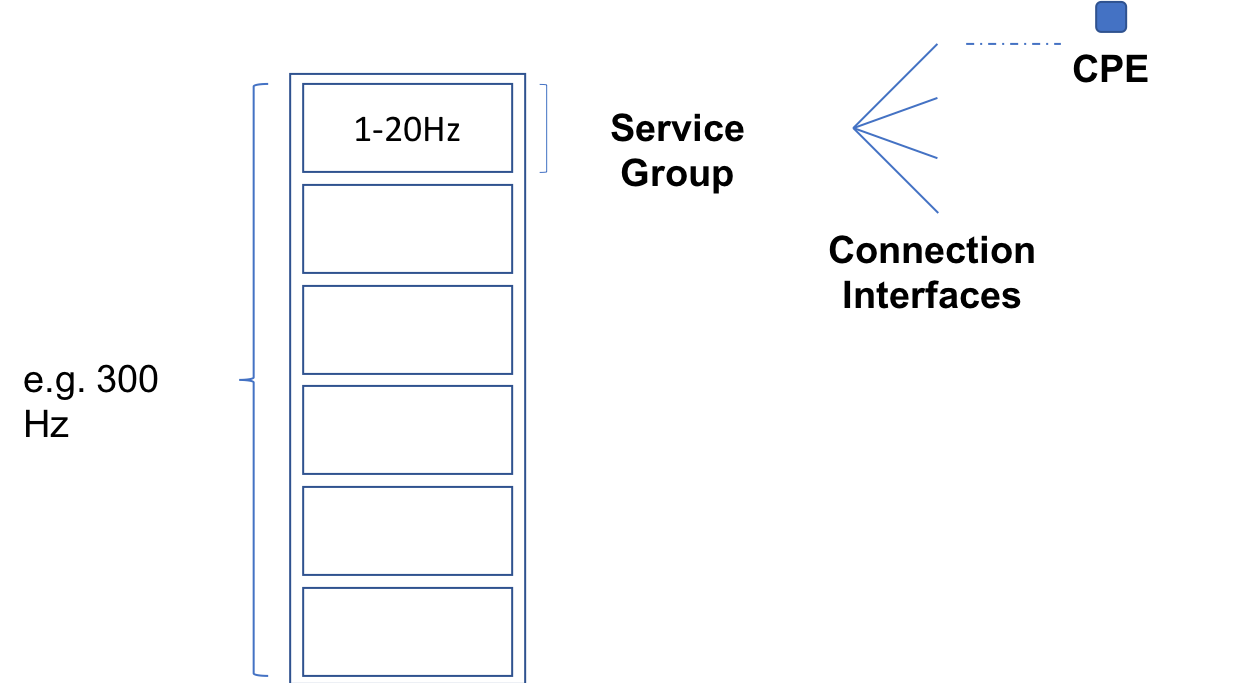
\includegraphics[width=0.5\linewidth]{SVG}
    \end{center}
    \caption{Details of the CMTS decomposition}
    \label{SVG}
\end{figure}

A CMTS splits the bandwidth it receives into multiple frequency ranges that are called Service Groups. A Service Group itself contains multiple connection interfaces as it can be observed in Figure~\ref{SVG}. Each CPE connects to a connection interface. The interface that is chosen depends on many parameters (e.g. load of the interface) and changes frequently. 

On the other hand, the association between a CPE and a service group does change as well but at a much slower rate (by order of days). 

\section{Problem Identified}
As opposed to some other providers, UPC owns the network it uses. Therefore the company has the opportunity to challenge the status quo. It has been polling regularly nodes of the network to perform passive operations. That gives it a myriad of possibilities to use all the data that is being collected but also future perspective of enriching it in order to build new tools and solutions.

As of today, the brand has trouble to understand customer behaviours. Because it cannot detect all problems if customers do not express any complaint, it cannot track how customers react to particular problems. As an example Teia Fetescu, a manager in THD\footnote{Technical help desk} Processes and Support Improvement, has expressed her frustration regarding how sometimes they witness a lot of complaints on social media about a particular problem but never received any calls regarding such problem and hence couldn't identify the symptoms and solve the problem. 

Therefore, we believe that we could leverage the data that UPC is using in order to identify CPEs that are failing and be able to do something about it. By having the capability to detect such problems the company could: go from passive to proactive troubleshooting, analyse how their customer reacts to given problems, and diagnose faster recurring problems.

\section{Data Sources}
As mentioned earlier, UPC collects a lot of data from its network in order to be able to troubleshoot problems, monitor its state, etc. We won't discuss all the data sources that have been used to fetch some minor information used along this project but rather give the two initial and main sources that were identified to be potentially leveraged by machine learning algorithms. As we should explain it in Section~\ref{sec:setup}, we will use data that is already being collected by UPC for different business needs:

\begin{itemize}
	\item ServAssure (SAA): Every 15 minutes, CMTS interfaces and CPEs are polled. Multiple measurements are monitored by such polling (e.g. Sound to Noise ratio, transmission power,...). Given the large number of such items it is impossible for UPC to keep a complete history of such polls. It aggregates them hourly and stores them for 11 days (10 full past days in addition to the current day). We would like to use this source in order to extract significant indicators of a CPE's Health.
	\item Virtual Interactive Assistant (VIA): interactions with the THD are tracked by the company in order to perform some reporting and also to be able to see a customer's history. This source is not very reliable as it depends on human interaction (the THD agent that answers the phone) with the software that helps them diagnose customers' problems. We were convinced that a proper filtering applied to this data would help us flag failing CPEs. It is important to note, though, that this isn't exactly flagging all the failing CPEs (e.g. some customers may not call the customer center when experiencing some problem).
\end{itemize}

\section{Setup of the Project}
\label{sec:setup}
First of all, it is important to note that this project was to the eyes of UPC a simple Proof of Concept that would help them determine the value that resides in the data that they own. This means that the support and resources available for conducting the project were fairly limited. 

As it is mentioned in the title, it was conducted inside the Data Management team. Members of the team have very limited knowledge concerning Data Analysis and Machine Learning. Nevertheless, because of their frequent interaction with the different data sources they had an overview of what data was available and how we could use it in order to build an innovative tool to answer business needs. Because of this framework, we had to reach out to different people in order to get help regarding the multiple components of this project:
\begin{itemize}
	\item Jonas Staempfli (\texttt{Jonas.Staempfli@upc.ch}): HFC support expert. Helped on understanding the network measurements and the way to use them in order to decide on the potential "failures" of CPEs.
	\item Felix Reisen (\texttt{Felix.Reisen@upc.ch}): Advanced Analytics inside the Business Intelligence team. Helped at supervising the different parts of the project from feasibility to implementation.
\end{itemize}

The project was realised during a heavy workload period and support proved to be a scarce resource. This is one of the points we will discuss before the conclusion, the knowledge regarding UPC’s business was complicated to obtain as it was detained by many different actors that may not have the time to deliver such piece of information. 

Finally, the POC was to use only the data that was already available as we couldn't afford (in terms of time nor budget) to organise the collection of new measurements on the CPE that could have been more helpful to diagnose.

\vspace{1\baselineskip}
The different terms are now introduced as well as the technical framework of the project. This should give the reader an understanding of the potential and challenges of this project. The final aim of the project should be clear ahead of this thesis as it will justify many choices and drive the research.

